\begin{figure}[ht]
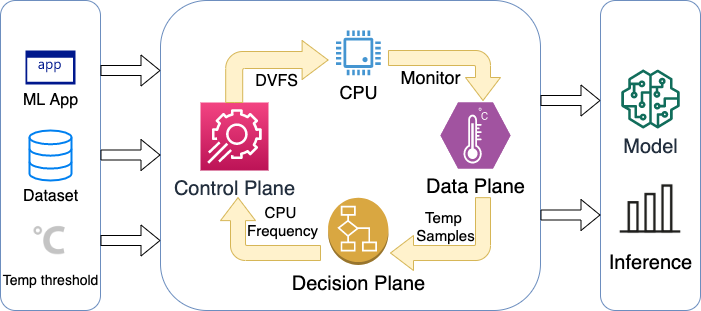
\includegraphics[width=\textwidth]{figures/Sparta.png}
\caption{The Architecture of Sparta} \label{fig:sparta}
\end{figure}

\subsection{Architecture}

To address the processor overheating challenge and accelerate the execution of applications under a CPU temperature threshold, we develop Sparta, a heat-budget-based scheduling framework for edge devices and machine learning applications. The architecture of Sparta is shown in Figure~\ref{fig:sparta}. The scheduler consists of three components: a control plane, a data plane, and a decision plane. Sparta takes a machine learning application, datasets, and a CPU temperature threshold as input. During the execution, the scheduler utilizes a feedback control mechanism that controls the CPU temperature by dynamically adjusting CPU frequency via system-level dynamic voltage and frequency scaling (DVFS). Sparta returns the trained model and inference results at the end of the execution. 


The data plane monitors, samples, and records the CPU real-time temperature via the lm-sensors interface~\cite{ref:sensors} and selects the maximum temperature within a sliding time window. Both the sampling rate and window size are configurable. (1/second and 5 seconds by default) To signify the authentic temperature of multi-core processors, data plane records the temperature samples of the entire CPU package instead of any specific ones. Being accessible by decision plane, all structured temperature data helps determine the proper CPU frequency in real time to keep the CPU temperature under threshold.

The control plane manages the CPU power and temperature. In the design phase, we consider two methods: Sleep injection and DVFS. The first method injects sleep time in the iteration loop that lowers the CPU usage, whereas the second method adjusts the CPU frequency by tuning the CPU voltage. We experiment with these two methods on a multi-threaded matrix multiplication benchmark and monitor the CPU temperature. Figure~\ref{fig:sleep} shows the CPU temperature time series using these two methods. We observe the latter method generates a controllable and stable temperature curve, and thus choose DVFS as the control plane interface. Upon the execution of scheduler, control plane receives the determined CPU frequency and sets the max clock speed of all cores in the CPU package on-the-fly. This way the control plane effectively manages the power consumption and heat generation of the processor.

\begin{figure}[ht]
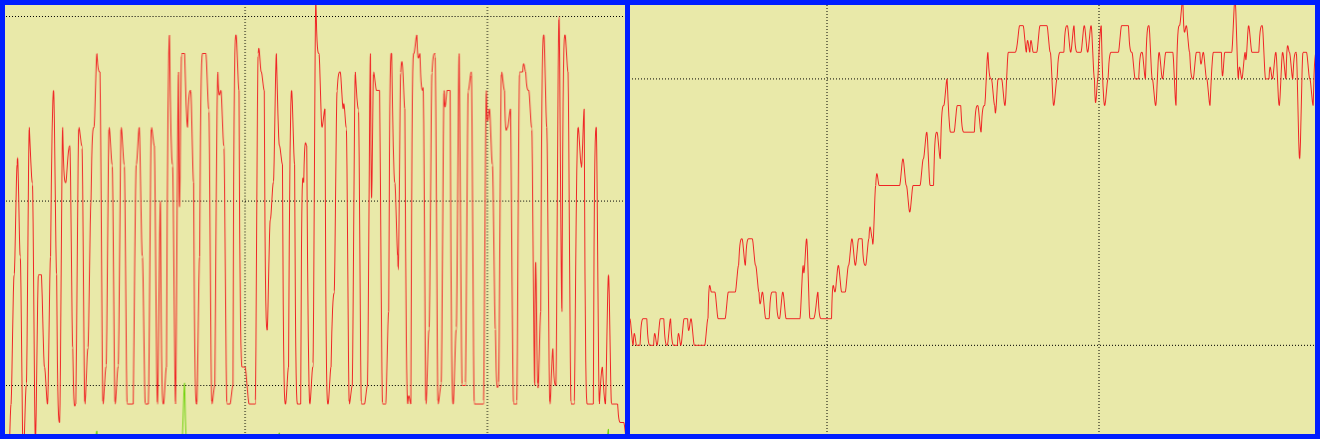
\includegraphics[width=\textwidth]{figures/Sleep-vs-dvfs.png}
\caption{The CPU temperature time series by sleep injection (left) vs DVFS (right). The x-axis is the time frame and the y-axis is the CPU temperature ranging from 48 \degree C to 100 \degree C. } \label{fig:sleep}
\end{figure}


The decision plane determines the CPU frequency based on historical and real-time temperature data throughout the execution. To provide the historical dataset, on which decision plane decides the initial CPU frequency, we collect CPU temperature and frequency data from a multi-threaded matrix multiplication (MATMUL) benchmark that simulates the underlying operations in machine learning applications. 

We gather the data in the ambient temperature ranging from 2.6 \degree C to 43.8 \degree C to cover different thermal environments. In the experiment, we found the sequence of CPU frequency and maximum temperature in a time window demonstrate a better linear relationship than the sequence of all temperature, because of its inherent oscillating feature. To verify the correlation between MATMUL and machine learning applications, we collect the same data from an image recognition application written in Tensorflow~\cite{ref:tensorflow}. As depicted in Figure~\ref{fig:mat-vs-tf}, we found the correlated linear relationship between the CPU frequency and logarithmic delta temperature defined as $log(T_{max} - T_i)$, where $T_{max}$ is the maximum temperature sample in the time window and $T_i$ is the starting CPU temperature in idle state. 
 
 Depending on this correlation, decision plane extrapolates the appropriate CPU frequency by linear regression from the MATMUL dataset and assigns initial CPU frequency before the execution starts. During the process, decision plane starts to extrapolate CPU frequency from real-time data that accurately reflects the ambient temperature and the execution pattern of ML applications. The extrapolation frequency is 12/minute by default and configurable by users.

\begin{figure}[ht]
\centering
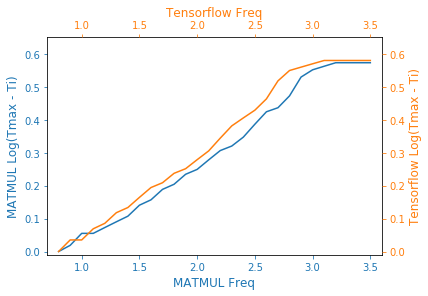
\includegraphics[scale=0.5]{figures/matmul-tensorflow.png}
\caption{The linear relationship between CPU frequency and logarithmic delta temperature of two benchmarks. The blue curve represents MATMUL and the orange curve represents the image recognition application. The plateaus at the right side of curves are caused by CPU hardware temperature throttling. } \label{fig:mat-vs-tf}
\end{figure}


\subsection{Operating Modes}

In the testing phase of Sparta, we identified two major problems in the decision plane. First, the extrapolation from linear regression oftentimes gets stuck at a local minimum. Thus, the determined CPU frequency is frequently lower than the ideal one, which leaves computational resources idle during execution. Second, the response time to correct the CPU from overheating is longer than expected when CPU temperature surpasses the threshold. To solve these two problems, we construct three operating modes for Sparta: Annealing, AIMD, and Hybrid. 

\subsubsection{Annealing} is a probabilistic algorithm that leverages the epsilon-greedy strategy that balances exploration and exploitation by choosing randomly. In this mode, Sparta scheduler picks a value(P) in the range [0, 1] uniformly at random and compares it with $\epsilon/K$, where $\epsilon$ is a probability of taking random actions (0.5 by default) and $K$ is the number of extrapolation decision plane has made. The scheduler assigns a random CPU frequency when P is greater, whereas it keeps the extrapolated frequency when P is less than $\epsilon/K$. With a decreasing probability of $\epsilon/K$ as the application proceeds, scheduler stabilizes and chooses to exploit what it has learned so far. When the ambient temperature or the execution pattern shifts dramatically, the scheduler resets the $\epsilon/K$ that allows more random exploration. This mode effectively addresses the problem of CPU frequency stuck at a local minimum and expedites the execution of machine learning applications under temperature threshold.

\subsubsection{AIMD} is a feedback control mechanism that responds to CPU temperature anomaly faster. The scheduler configures the CPU frequency according to the historical data extrapolation at the start of execution. During the execution, it decreases the CPU frequency by a multiplicative factor (0.5 by default) when CPU temperature surpasses the threshold. Subsequently, it increases the frequency by a fixed amount (0.07 GHz by default) every iteration until the CPU temperature stabilizes right below the threshold. The decision plane turns into hibernation at this point to prevent redundant tuning on CPU frequency that leads to inefficient execution. Meanwhile, the data plane keeps monitoring the CPU temperature and wakes up decision plane if any anomalies caused by ambient temperature or execution pattern are detected. AIMD reduces the response time to temperature deviation and keeps most samples under the threshold. 

\subsubsection{Hybrid} combines Annealing and AIMD modes to address each other's disadvantage: if the probabilistic actions in Annealing drive CPU temperature above threshold, AIMD brings the anomaly back to normal fast; when AIMD settles at a local minimum of CPU frequency and leaves resources idle, Annealing boosts the execution by assigning a random CPU frequency. This way, Hybrid mode provides a complement to accelerate the machine learning execution while keeping the CPU temperature under threshold. 
